\chapter{The predictive soundscape model framework and a proposal for future models}
  \label{ch:bayes}
% alt:A Bayesian Hierarchical Predictive Soundscape Model and a Proposed Soundscape Index
% alt: Probabilistic soundscape models including personal, contextual, environmental, and acoustic information

\section{Introduction}
\subsection{The problem with the pleasant-annoying paradigm}

As made clear by their name, noise annoyance studies have focussed on the relationship between noise (or acoustic) features and the perceived annoyance, to varying degrees of success. Within the soundscape circumplex framework, annoyance is the negative side of the pleasantness dimension, forming the \nth{1} primary component of soundscape perception. This means that, along with pleasantness, annoyance is that perceptual attribute which is most readily perceived and plays the largest part in differentiating between the perception of different soundscapes. This fact therefore makes this pleasantness dimension the prime target for addressing noise issues. 

However, \citet{Mitchell2021Investigating} (i.e. \cref{ch:lockdown}) and \citet{Aumond2022} have both recently demonstrated a fundamental difference in the statistical relationships connecting context and acoustic features with the perceived pleasantness and eventfulness of urban soundscapes. %TODO: Continue this discussion about including eventfulness. Can draw from that review I wrote

\section{Defining the predictive soundscape model framework}

\subsection{Goals}
Before defining what form a practical predictive model should take, we first need to make clear what the goals of such a model is. First, that it to a reasonable extent is successful in predicting the collective perception of a soundscape. Per \cref{ch:circumplex}, it should succeed at both indicating the central tendency of the soundscape perception, but importantly it should also inform the likely spread of perception among the population. In other words, ideally the model will result in an accurate soundscape shape within the circumplex. Second, that it can be applied to unmanned uses, such as smart city sensors and soundscape mapping. It is impractical to conduct soundscape surveys or soundwalks in every location we wish to map and certainly not when we wish to see how these locations change over longer periods of time. A predictive model should allow us to survey these soundscapes remotely. Third, the model should enable us to test and score proposed interventions. In a design context, it is crucial that various design strategies and interventions can be tested and that the influencing factors can be identified. The model should assist the user in highlighting what factor is limiting the success of a soundscape, spark ideas for how to address it, and allow these ideas to be tested. Several other useful features of predictive soundscape models arise out of these goals and will be discussed later, but these form the core goals of the framework.

\subsection{Constraints}
If we accept that predictive models are necessary to advance a more holistic approach to urban sound in smart cities, we must then define the constraints of such a model. The goal here is to define a framework for what is needed from a future model intended to be used in a smart city sensors, soundscape mapping, or urban design context.

The first constraint is that the model must be based on measurable factors. By this, I mean the data which feeds into the predictive model should be collected via measurements of one sort or another; this could be acoustic sound level measurements or recordings, environmental measurements, video recordings, or GIS measurements, etc.. What it certainly cannot include is perceptual data. This is strictly a practical constraint - for a predictive model designed to be used in practice, there is no justification to include other perceptual factors derived from surveys but not whichever factor you desire to predict. If the goal is to predict soundscape pleasantness and it is necessary to survey people about the visual pleasantness, why not just also survey them about the soundscape pleasantness directly? Certainly this mix of perceptual data is useful in research and can elucidate the relationships between the sonic and visual environments, but it is not useful in a practical predictive context. Any results which arise from research combining this sort of perceptual information must eventually be translated into a component which can itself be measured or modelled. 

The second constraint is that any analysis of the measured data can be done automatically, without human intervention. If the eventual goal is to deploy the model on continuously-running, unmanned sensor nodes or to enable practical large-scale measurements, the predictive model should be capable of operating with minimal human input. This means, for instance, that if the model includes information about the sound source, this identification of the source should be possible to do automatically (i.e. through environmental sound recognition). This is in contrast to the type of analysis done in \cref{ch:mlmann} where the sound sources were identified manually by the researchers. 

The third constraint is for the model to be generalisable to new locations. Ideally, it will be generalisable to new and (to it) unfamiliar soundscape types, but the minimum requirement should be that it can be applied to new locations which are otherwise similar to those in the training data. This means that any factors which are used to characterise the context provided by the location should be distinguished from a simple label of the location and should instead be derived from measurements of the location. In practice this could be geographical or architectural characteristics of the space, a proposed use-case of the space, or consistent visual characteristics of the space such as the proportion of pavement to green elements. This is in contrast to the model created for \cref{ch:lockdown} which was constrained to be used only on those locations included in the training data since it made use of a location label.

For this third point, some aspects of the second constraint can be relaxed. Since this would only need to be defined once for a location, definitions such as the use case of the space could be defined by the person using the model. What is necessary is that the model and its component location-context factors can be set up ahead of time by the user, then the recording-level effects are able to be calculated automatically. In the MLM context this essentially amounts to choosing the appropriate location-level coefficients ahead of time then automatically calculating the features which are fed into those coefficients (per constraint 1).

Finally, the model should be robust to missing components. If the original or full construction of the model depends on demographic information of the population using the space, in cases where this information is not available, it should be possible to omit it and still obtain a reasonable result. Here we may define potential `must-have’ and `optional’ factors. Given the amount of variance explained by the various factors explored in this thesis, in-depth acoustic information is a must-have, while demographic and personal factors are an optional factor where the trade-off of losing 3\% of the explained variance in eventfulness (as shown in \cref{ch:whostudy}) is accepted as reasonable. Based on the results of \cref{ch:lockdown}, it would appear that location-context is crucial for modelling the pleasantness, but not for modelling the eventfulness. In order to determine the must-have factors for characterising the location-context, more work will need to be done to determine the appropriate input factors and their relative importance. The first step of this is bringing the model in line with constraint 3. 


\section{Starting point}

To illustrate how a model which fits this proposed framework could be developed, I will start with the model presented in \cref{ch:lockdown} and build upon it. Each of the three models presented in this thesis forms some component of the ideal final model and addresses one constraint or another, but the \cref{ch:lockdown} model was the most developed and most successful so we take it as the starting point. 

\subsection{Where it stands}

As it is, this model violates most obviously violates constraint 3 - it is not generalisable to new locations. Since the structure of the \gls{mlm} has the `LocationID' as the categorical feature used in the second level, any new data must be able to conform to one of the original 13 locations. Technically, it would be possible to select the location in the training data which is considered most similar to the new location and use the coefficients derived for it, but this is a poor design for a generalisable model. 

\section{Incorporating personal factors into a predictive soundscape model}
Although, as \citet{Droumeva2021sound} points out, each individual brings their own cultural and subjective aspects of listening to the stage of urban sound, when attempting to characterise the soundscape of a space, it is not a particular individual's aspects we should be concerned with. That individual forms a part of the collective perception of the space. Their cultural and subjective (i.e. personal) aspects mitigate their perception, but this perception then forms only a single component of the collective perception. How then should we consider these personal factors? Surely there is no suggestion to disregard their influence and importance within the soundscape approach? In my view, there are two approaches:

\begin{enumerate}
  \item Incorporate these personal factors as demographic statistics of a location; or
  \item An agent-based approach where each individual likely to use the space is simulated and modelled with their personal factors to then be included in the collective perception.
\end{enumerate}

Let's look at how these two approaches would be implemented in a multilevel acoustics-based predictive model, such as those presented in \crefrange{ch:mlmann}{ch:lockdown}.

%TODO: Expand
\subsection{Approach 1}
In the first, the demographic breakdown of the space under investigation is estimated, either through a census or by the designers' desired use case. This demographic breakdown can then be compared to the results presented above \citep{Erfanian2021Psychological} to derive weighting factors which adjust the predicted soundscape assessment. For instance, the results suggest that retired persons perceive the soundscape as \draft{XX\% or amount [need to check with results]} less pleasant than others. If the particular space under investigation has a large proportion of retired persons, say 65\% we could then apply an adjustment to the initial personal-factors-agnostic prediction to reflect this tendency. In this example, an initial location-level \gls{isopl} prediction of 0.36, with a 65\% retired population would be corrected by \draft{-XX [0.65 x result]} for a final demographics-corrected \gls{isopl} prediction of \draft{XX}.

\subsection{Approach 2}

\subsection{Benefits and downsides of each approach}

\section{Incorporating sound source information}

\section{Probabilistic predictions - A Bayesian Approach?}

Goal number 1 presents perhaps the most difficult future challenge. The starting point model from \cref{ch:lockdown} was successful in predicting the central tendency (i.e. mean response) of the soundscape of the locations, but it failed to accurately reflect the distribution of responses within the locations. Since the \gls{mlm} used is frequentist, the expectation is that each set of inputs has one `true' output and any deviation from this represents the error factor of the model. This view (one input = one output) is in contrast to the view put forward by the representations proposed in \cref{ch:circumplex}. When considering a collective perception, it is unreasonable to expect that any given input (i.e. a single recording) will have a single `correct' response. People will perceive the same sound differently. Regardless of how precisely we can characterise the person or population in terms of their personal factors or the context surrounding it, there is no single response to a given sound, instead we should expect to see a distribution of responses. 

By pulling from data collected as part of the \gls{satp}, we can investigate the expected spread of responses to the same sound. In this study, respondents across the world were exposed to a curated set of 27 binaural recordings and responded according to the \gls{ssqp} survey. %TODO: Return here 

\subsection{Defining a distribution}

\subsubsection{Truncated normal distribution}

Given that the \gls{isopl} and \gls{isoev} values have a hard boundary at $[-1, +1]$, it is not in fact correct to consider the distribution of responses within the circumplex as a normal distribution. A normal distribution is defined as extending out to $(-\infty, \infty)$ with an area of 1 under the probability density. If the potential space of the responses is bounded, the assumption of them forming a normal distribution is violated, as part of the probability density function is unreachable, meaning the area under the probability density will not sum to 1.

If we assume the general shape of the responses to be normal, then they would instead form a truncated normal distribution \cit{\url{https://people.sc.fsu.edu/~jburkardt/presentations/truncated_normal.pdf}, \url{https://www.tandfonline.com/doi/abs/10.1080/00031305.1999.10474490}}. Briefly, a truncated normal distribution is estimated by first calculating the probability density function of the standard normal distribution. Then, the density function is truncated at the set boundary ($[a, \infty)$ or $(-\infty, b]$) or boundaries ($[a, b]$) and the portion of the density function which is truncated is redistributed within the boundary.

This redistribution means that the various parameters of a truncated distribution will be somewhat different than for a normal distribution, in particular the calculation of variance. This impacts the soundscape distribution plots demonstrated in \cref{ch:circumplex} as the kernel density estimation performed by the underlying plotting library (\texttt{seaborn}) assumes a normal distribution with no boundary. It is possible that making use of a truncated normal distribution would change the shape of the distributions produced by \texttt{soundscapy}. Although at this point there does not seem to be a simple method of adapting the \texttt{soundscapy} code to make use of a truncated distribution, I chose to briefly test out how much of a change the truncated distribution is likely to make to the shape of the \texttt{soundscapy} plots through functions available in \texttt{R}. 

\begin{figure}
  \centering
  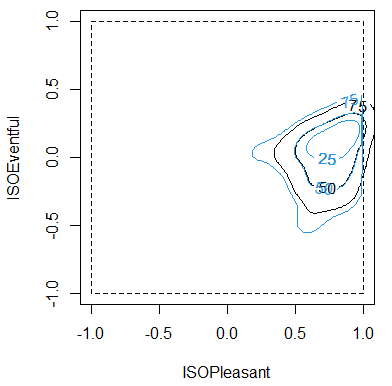
\includegraphics{Figures/Trunc-Normal-demo.png}
  \caption{Comparing a probability distribution in the soundscape circumplex (using Regents Park Japan as the worst case example) using a normal kernel density estimation method (black line) and a truncated KDE (blue line). \label{fig:truncatekde}}
\end{figure}

From \cref{fig:truncatekde}, it appears that there would be some difference in the shape of the soundscape distribution when using a truncated distribution. However, I would note that Regents Park Japan was chosen as the worst case location in the whole \gls{isd} as the samples lie closest to the boundary and the density function estimated in \texttt{soundscapy} has the most area which lies outside the boundary. Most locations do not show any overlap with the boundary and would not be noticeably affected by the truncation. In addition, switching to the truncated normal distribution only affects those iso-density levels which overlap with the boundary. Therefore, the recommended simplified density curve given in \cref{ch:circumplex} of 50\% is effectively unchanged since it is very unlikely the \nth{50} percentile curve would exceed the boundaries. For the time-being, therefore it appears that there is not a detriment to using a standard normal distribution as opposed to a truncated normal distribution, for the visualisations created by \texttt{soundscapy}.

However, as I move towards a probabilistic prediction framework, and even in the frequentist predictive models used throughout this thesis, it seems possible that the distinctions between these underlying distributions will become more important. 


\section{Discussion}

\section{Conclusion}

